% Options for packages loaded elsewhere
\PassOptionsToPackage{unicode}{hyperref}
\PassOptionsToPackage{hyphens}{url}
%
\documentclass[
]{article}
\usepackage{amsmath,amssymb}
\usepackage{lmodern}
\usepackage{iftex}
\ifPDFTeX
  \usepackage[T1]{fontenc}
  \usepackage[utf8]{inputenc}
  \usepackage{textcomp} % provide euro and other symbols
\else % if luatex or xetex
  \usepackage{unicode-math}
  \defaultfontfeatures{Scale=MatchLowercase}
  \defaultfontfeatures[\rmfamily]{Ligatures=TeX,Scale=1}
\fi
% Use upquote if available, for straight quotes in verbatim environments
\IfFileExists{upquote.sty}{\usepackage{upquote}}{}
\IfFileExists{microtype.sty}{% use microtype if available
  \usepackage[]{microtype}
  \UseMicrotypeSet[protrusion]{basicmath} % disable protrusion for tt fonts
}{}
\makeatletter
\@ifundefined{KOMAClassName}{% if non-KOMA class
  \IfFileExists{parskip.sty}{%
    \usepackage{parskip}
  }{% else
    \setlength{\parindent}{0pt}
    \setlength{\parskip}{6pt plus 2pt minus 1pt}}
}{% if KOMA class
  \KOMAoptions{parskip=half}}
\makeatother
\usepackage{xcolor}
\usepackage[margin=1in]{geometry}
\usepackage{color}
\usepackage{fancyvrb}
\newcommand{\VerbBar}{|}
\newcommand{\VERB}{\Verb[commandchars=\\\{\}]}
\DefineVerbatimEnvironment{Highlighting}{Verbatim}{commandchars=\\\{\}}
% Add ',fontsize=\small' for more characters per line
\usepackage{framed}
\definecolor{shadecolor}{RGB}{248,248,248}
\newenvironment{Shaded}{\begin{snugshade}}{\end{snugshade}}
\newcommand{\AlertTok}[1]{\textcolor[rgb]{0.94,0.16,0.16}{#1}}
\newcommand{\AnnotationTok}[1]{\textcolor[rgb]{0.56,0.35,0.01}{\textbf{\textit{#1}}}}
\newcommand{\AttributeTok}[1]{\textcolor[rgb]{0.77,0.63,0.00}{#1}}
\newcommand{\BaseNTok}[1]{\textcolor[rgb]{0.00,0.00,0.81}{#1}}
\newcommand{\BuiltInTok}[1]{#1}
\newcommand{\CharTok}[1]{\textcolor[rgb]{0.31,0.60,0.02}{#1}}
\newcommand{\CommentTok}[1]{\textcolor[rgb]{0.56,0.35,0.01}{\textit{#1}}}
\newcommand{\CommentVarTok}[1]{\textcolor[rgb]{0.56,0.35,0.01}{\textbf{\textit{#1}}}}
\newcommand{\ConstantTok}[1]{\textcolor[rgb]{0.00,0.00,0.00}{#1}}
\newcommand{\ControlFlowTok}[1]{\textcolor[rgb]{0.13,0.29,0.53}{\textbf{#1}}}
\newcommand{\DataTypeTok}[1]{\textcolor[rgb]{0.13,0.29,0.53}{#1}}
\newcommand{\DecValTok}[1]{\textcolor[rgb]{0.00,0.00,0.81}{#1}}
\newcommand{\DocumentationTok}[1]{\textcolor[rgb]{0.56,0.35,0.01}{\textbf{\textit{#1}}}}
\newcommand{\ErrorTok}[1]{\textcolor[rgb]{0.64,0.00,0.00}{\textbf{#1}}}
\newcommand{\ExtensionTok}[1]{#1}
\newcommand{\FloatTok}[1]{\textcolor[rgb]{0.00,0.00,0.81}{#1}}
\newcommand{\FunctionTok}[1]{\textcolor[rgb]{0.00,0.00,0.00}{#1}}
\newcommand{\ImportTok}[1]{#1}
\newcommand{\InformationTok}[1]{\textcolor[rgb]{0.56,0.35,0.01}{\textbf{\textit{#1}}}}
\newcommand{\KeywordTok}[1]{\textcolor[rgb]{0.13,0.29,0.53}{\textbf{#1}}}
\newcommand{\NormalTok}[1]{#1}
\newcommand{\OperatorTok}[1]{\textcolor[rgb]{0.81,0.36,0.00}{\textbf{#1}}}
\newcommand{\OtherTok}[1]{\textcolor[rgb]{0.56,0.35,0.01}{#1}}
\newcommand{\PreprocessorTok}[1]{\textcolor[rgb]{0.56,0.35,0.01}{\textit{#1}}}
\newcommand{\RegionMarkerTok}[1]{#1}
\newcommand{\SpecialCharTok}[1]{\textcolor[rgb]{0.00,0.00,0.00}{#1}}
\newcommand{\SpecialStringTok}[1]{\textcolor[rgb]{0.31,0.60,0.02}{#1}}
\newcommand{\StringTok}[1]{\textcolor[rgb]{0.31,0.60,0.02}{#1}}
\newcommand{\VariableTok}[1]{\textcolor[rgb]{0.00,0.00,0.00}{#1}}
\newcommand{\VerbatimStringTok}[1]{\textcolor[rgb]{0.31,0.60,0.02}{#1}}
\newcommand{\WarningTok}[1]{\textcolor[rgb]{0.56,0.35,0.01}{\textbf{\textit{#1}}}}
\usepackage{graphicx}
\makeatletter
\def\maxwidth{\ifdim\Gin@nat@width>\linewidth\linewidth\else\Gin@nat@width\fi}
\def\maxheight{\ifdim\Gin@nat@height>\textheight\textheight\else\Gin@nat@height\fi}
\makeatother
% Scale images if necessary, so that they will not overflow the page
% margins by default, and it is still possible to overwrite the defaults
% using explicit options in \includegraphics[width, height, ...]{}
\setkeys{Gin}{width=\maxwidth,height=\maxheight,keepaspectratio}
% Set default figure placement to htbp
\makeatletter
\def\fps@figure{htbp}
\makeatother
\setlength{\emergencystretch}{3em} % prevent overfull lines
\providecommand{\tightlist}{%
  \setlength{\itemsep}{0pt}\setlength{\parskip}{0pt}}
\setcounter{secnumdepth}{-\maxdimen} % remove section numbering
\ifLuaTeX
  \usepackage{selnolig}  % disable illegal ligatures
\fi
\IfFileExists{bookmark.sty}{\usepackage{bookmark}}{\usepackage{hyperref}}
\IfFileExists{xurl.sty}{\usepackage{xurl}}{} % add URL line breaks if available
\urlstyle{same} % disable monospaced font for URLs
\hypersetup{
  pdftitle={Classification Competition Code},
  hidelinks,
  pdfcreator={LaTeX via pandoc}}

\title{Classification Competition Code}
\author{}
\date{\vspace{-2.5em}14 March 2023}

\begin{document}
\maketitle

\hypertarget{loading-packages}{%
\section{Loading Packages}\label{loading-packages}}

\hypertarget{pre-processing}{%
\section{Pre-processing}\label{pre-processing}}

\begin{Shaded}
\begin{Highlighting}[]
\FunctionTok{set.seed}\NormalTok{(}\DecValTok{1}\NormalTok{)}

\CommentTok{\# Load data}
\CommentTok{\#download.file(\textquotesingle{}https://github.com/lse{-}my474/pset\_data/raw/main/coms\_tr.csv\textquotesingle{}, \textquotesingle{}coms\_tr.csv\textquotesingle{})}
\CommentTok{\#download.file(\textquotesingle{}https://github.com/lse{-}my474/pset\_data/raw/main/coms\_te.csv\textquotesingle{}, \textquotesingle{}coms\_te.csv\textquotesingle{})}
\NormalTok{coms\_te }\OtherTok{\textless{}{-}} \FunctionTok{read.csv}\NormalTok{(}\StringTok{\textquotesingle{}coms\_te.csv\textquotesingle{}}\NormalTok{, }\AttributeTok{stringsAsFactors =}\NormalTok{ F)}
\NormalTok{coms\_tr }\OtherTok{\textless{}{-}} \FunctionTok{read.csv}\NormalTok{(}\StringTok{\textquotesingle{}coms\_tr.csv\textquotesingle{}}\NormalTok{, }\AttributeTok{stringsAsFactors =}\NormalTok{ F)}

\NormalTok{coms\_tr }\SpecialCharTok{\%\textgreater{}\%}
  \FunctionTok{group\_by}\NormalTok{(toxic) }\SpecialCharTok{\%\textgreater{}\%}
  \FunctionTok{summarise}\NormalTok{(}\AttributeTok{count =} \FunctionTok{n}\NormalTok{())}
\end{Highlighting}
\end{Shaded}

\begin{verbatim}
## # A tibble: 2 x 2
##   toxic  count
##   <int>  <int>
## 1     0 113067
## 2     1  14681
\end{verbatim}

\begin{Shaded}
\begin{Highlighting}[]
\CommentTok{\# wrangle for compatibility }
\NormalTok{coms\_te}\SpecialCharTok{$}\NormalTok{sample }\OtherTok{\textless{}{-}} \FunctionTok{rep}\NormalTok{(}\StringTok{\textquotesingle{}test\textquotesingle{}}\NormalTok{, }\FunctionTok{nrow}\NormalTok{(coms\_te))}
\NormalTok{coms\_te}\SpecialCharTok{$}\NormalTok{toxic }\OtherTok{\textless{}{-}} \FunctionTok{rep}\NormalTok{(}\ConstantTok{NA}\NormalTok{, }\FunctionTok{nrow}\NormalTok{(coms\_te))}
\NormalTok{coms\_tr}\SpecialCharTok{$}\NormalTok{sample }\OtherTok{\textless{}{-}} \FunctionTok{rep}\NormalTok{(}\StringTok{\textquotesingle{}train\textquotesingle{}}\NormalTok{, }\FunctionTok{nrow}\NormalTok{(coms\_tr))}

\CommentTok{\# Create full df}
\NormalTok{data }\OtherTok{\textless{}{-}} \FunctionTok{rbind}\NormalTok{(coms\_tr, coms\_te)}

\CommentTok{\# Create Corpus}
\NormalTok{corpus }\OtherTok{\textless{}{-}} \FunctionTok{corpus}\NormalTok{(data, }\AttributeTok{text\_field=}\StringTok{"comment"}\NormalTok{)}

\DocumentationTok{\#\#\#\#\#\#\#\#\#\#\#\#\# Create tokens}

\CommentTok{\# 1 to 3 word n{-}grams. Vastly increases sparseness as data as p increases, so must be aware of this when selecting a model. }
\CommentTok{\# all to lower for matching, removing stopwords.}
\CommentTok{\# manual\_words vector refers to words that appear in both toxic and non{-}toxic posts and can not be used to identify either. }

\NormalTok{manual\_words }\OtherTok{\textless{}{-}} \FunctionTok{c}\NormalTok{(}\StringTok{\textquotesingle{}page\textquotesingle{}}\NormalTok{, }\StringTok{\textquotesingle{}edit\textquotesingle{}}\NormalTok{, }\StringTok{\textquotesingle{}wikipedia\textquotesingle{}}\NormalTok{, }\StringTok{\textquotesingle{}like\textquotesingle{}}\NormalTok{, }\StringTok{\textquotesingle{}articl\textquotesingle{}}\NormalTok{, }\StringTok{\textquotesingle{}just\textquotesingle{}}\NormalTok{,}\StringTok{\textquotesingle{}use\textquotesingle{}}\NormalTok{)}

\NormalTok{toks\_ngrams }\OtherTok{\textless{}{-}}  \FunctionTok{tokens}\NormalTok{(corpus, }\AttributeTok{remove\_punct =} \ConstantTok{TRUE}\NormalTok{)}\SpecialCharTok{\%\textgreater{}\%}
  \FunctionTok{tokens\_tolower}\NormalTok{() }\SpecialCharTok{\%\textgreater{}\%}
  \FunctionTok{tokens\_remove}\NormalTok{(}\AttributeTok{pattern =} \FunctionTok{c}\NormalTok{(}\FunctionTok{stopwords}\NormalTok{(}\StringTok{"english"}\NormalTok{), }\FunctionTok{c}\NormalTok{(}\StringTok{"="}\NormalTok{,}\StringTok{"\textasciigrave{}"}\NormalTok{, }\StringTok{"\textasciitilde{}"}\NormalTok{, }\StringTok{"|"}\NormalTok{, }\StringTok{":"}\NormalTok{)), }\AttributeTok{padding =} \ConstantTok{FALSE}\NormalTok{) }\SpecialCharTok{\%\textgreater{}\%}
  \FunctionTok{tokens}\NormalTok{(}\AttributeTok{remove\_punct =} \ConstantTok{TRUE}\NormalTok{, }\AttributeTok{remove\_numbers =} \ConstantTok{TRUE}\NormalTok{, }\AttributeTok{remove\_symbols =} \ConstantTok{TRUE}\NormalTok{) }\SpecialCharTok{\%\textgreater{}\%}
  \FunctionTok{tokens\_wordstem}\NormalTok{(}\AttributeTok{language =} \FunctionTok{quanteda\_options}\NormalTok{(}\StringTok{"language\_stemmer"}\NormalTok{)) }\SpecialCharTok{\%\textgreater{}\%}
  \FunctionTok{tokens\_remove}\NormalTok{(manual\_words, }\AttributeTok{padding =} \ConstantTok{TRUE}\NormalTok{) }\SpecialCharTok{\%\textgreater{}\%}
  \FunctionTok{tokens\_ngrams}\NormalTok{(}\DecValTok{1}\SpecialCharTok{:}\DecValTok{2}\NormalTok{)}

\DocumentationTok{\#\#\#\#\#\#\#\#\#\#\#\#\# Create dfm}

\CommentTok{\# initialising df }
\NormalTok{dfm\_draft }\OtherTok{\textless{}{-}} \FunctionTok{dfm}\NormalTok{(toks\_ngrams)}

\CommentTok{\# set word frequency limit on dfm to trim to most relevant features (selection). }
\NormalTok{dfm\_trimmed }\OtherTok{\textless{}{-}} \FunctionTok{dfm\_trim}\NormalTok{(dfm\_draft, }\AttributeTok{min\_docfreq =} \DecValTok{75}\NormalTok{)}

\CommentTok{\# final dfm}
\NormalTok{dfm\_final }\OtherTok{\textless{}{-}}\NormalTok{ dfm\_trimmed}
\end{Highlighting}
\end{Shaded}

\hypertarget{feature-selection-with-tf-idf}{%
\section{Feature Selection with
TF-IDF}\label{feature-selection-with-tf-idf}}

\begin{Shaded}
\begin{Highlighting}[]
\FunctionTok{set.seed}\NormalTok{(}\DecValTok{1}\NormalTok{)}

\NormalTok{tfidf\_data }\OtherTok{\textless{}{-}} \FunctionTok{dfm\_tfidf}\NormalTok{(dfm\_final, }\AttributeTok{scheme\_tf =} \StringTok{\textquotesingle{}prop\textquotesingle{}}\NormalTok{)}

\NormalTok{tfidf\_col\_means }\OtherTok{\textless{}{-}} \FunctionTok{colMeans}\NormalTok{(tfidf\_data)}

\FunctionTok{hist}\NormalTok{(tfidf\_col\_means, }\AttributeTok{breaks =} \DecValTok{40}\NormalTok{, }\AttributeTok{main =} \StringTok{"Distribution of Column Means"}\NormalTok{, }\AttributeTok{xlab =} \StringTok{"Column Means"}\NormalTok{)}
\end{Highlighting}
\end{Shaded}

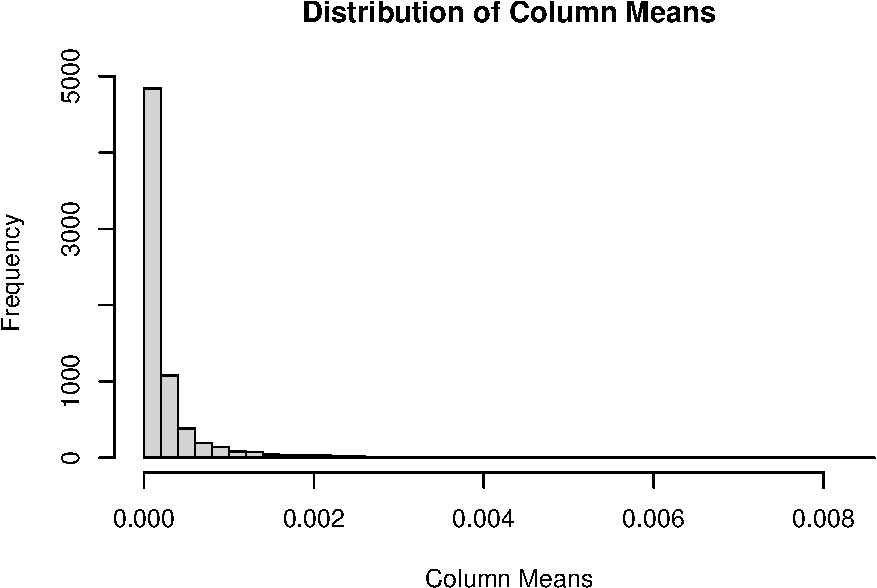
\includegraphics{classifier_files/figure-latex/tfidf-1.pdf}

\begin{Shaded}
\begin{Highlighting}[]
\NormalTok{zero\_tfidf }\OtherTok{\textless{}{-}} \FunctionTok{which}\NormalTok{(tfidf\_col\_means }\SpecialCharTok{\textless{}=} \FloatTok{0.0001}\NormalTok{)}

\FunctionTok{length}\NormalTok{(zero\_tfidf)}
\end{Highlighting}
\end{Shaded}

\begin{verbatim}
## [1] 3034
\end{verbatim}

\begin{Shaded}
\begin{Highlighting}[]
\NormalTok{zero\_tfidf\_names }\OtherTok{=} \FunctionTok{names}\NormalTok{(zero\_tfidf)}

\FunctionTok{paste}\NormalTok{(}\StringTok{"There are"}\NormalTok{, }\FunctionTok{ncol}\NormalTok{(dfm\_final), }\StringTok{"features before filtering via tfidf."}\NormalTok{)}
\end{Highlighting}
\end{Shaded}

\begin{verbatim}
## [1] "There are 7018 features before filtering via tfidf."
\end{verbatim}

\begin{Shaded}
\begin{Highlighting}[]
\CommentTok{\# removing obsolete tokens}
\NormalTok{dfm\_final }\OtherTok{\textless{}{-}}\NormalTok{ dfm\_final }\SpecialCharTok{\%\textgreater{}\%}
  \FunctionTok{dfm\_remove}\NormalTok{(}\AttributeTok{pattern =}\NormalTok{ zero\_tfidf\_names)}

\CommentTok{\# removing tokens beginning with numbers}
\NormalTok{manual\_words\_2 }\OtherTok{\textless{}{-}} \FunctionTok{c}\NormalTok{(}\StringTok{"2nd"}\NormalTok{, }\StringTok{"wp:ani"}\NormalTok{)}

\NormalTok{dfm\_final }\OtherTok{\textless{}{-}}\NormalTok{ dfm\_final }\SpecialCharTok{\%\textgreater{}\%}
  \FunctionTok{dfm\_remove}\NormalTok{(}\AttributeTok{pattern =}\NormalTok{ manual\_words\_2)}

\FunctionTok{paste}\NormalTok{(}\StringTok{"There are"}\NormalTok{, }\FunctionTok{ncol}\NormalTok{(dfm\_final), }\StringTok{"features after filtering via tfidf."}\NormalTok{)}
\end{Highlighting}
\end{Shaded}

\begin{verbatim}
## [1] "There are 3982 features after filtering via tfidf."
\end{verbatim}

\begin{Shaded}
\begin{Highlighting}[]
\DocumentationTok{\#\#\#\#\#\#\#\#\#\#\#\#\# Create test and train dfm sets.}
\NormalTok{train\_dfm }\OtherTok{\textless{}{-}}\NormalTok{ dfm\_final[dfm\_final}\SpecialCharTok{$}\NormalTok{sample }\SpecialCharTok{==} \StringTok{\textquotesingle{}train\textquotesingle{}}\NormalTok{,]}
\NormalTok{test\_dfm }\OtherTok{\textless{}{-}}\NormalTok{ dfm\_final[dfm\_final}\SpecialCharTok{$}\NormalTok{sample }\SpecialCharTok{==} \StringTok{\textquotesingle{}test\textquotesingle{}}\NormalTok{,]}
\end{Highlighting}
\end{Shaded}

\hypertarget{feature-selection-and-modelling-with-lasso}{%
\section{Feature Selection and Modelling with
LASSO}\label{feature-selection-and-modelling-with-lasso}}

\begin{Shaded}
\begin{Highlighting}[]
\FunctionTok{set.seed}\NormalTok{(}\DecValTok{1}\NormalTok{)}

\CommentTok{\# nlambda = 200 rather than 101, increases certainty that this lambda is proper minimum {-} this is a surrogate learning rate.}
\NormalTok{lasso\_cv }\OtherTok{\textless{}{-}} \FunctionTok{cv.glmnet}\NormalTok{(}\AttributeTok{x =}\NormalTok{ train\_dfm,}
                   \AttributeTok{y =} \FunctionTok{docvars}\NormalTok{(train\_dfm)}\SpecialCharTok{$}\NormalTok{toxic,}
                   \AttributeTok{family=}\StringTok{"binomial"}\NormalTok{,}
                   \AttributeTok{alpha=}\DecValTok{1}\NormalTok{,}
                   \AttributeTok{nfolds=}\DecValTok{5}\NormalTok{,}
                   \AttributeTok{nlambda =} \DecValTok{200}\NormalTok{,}
                   \AttributeTok{maxit =} \DecValTok{10000}\NormalTok{)}

\FunctionTok{plot}\NormalTok{(lasso\_cv)}
\end{Highlighting}
\end{Shaded}

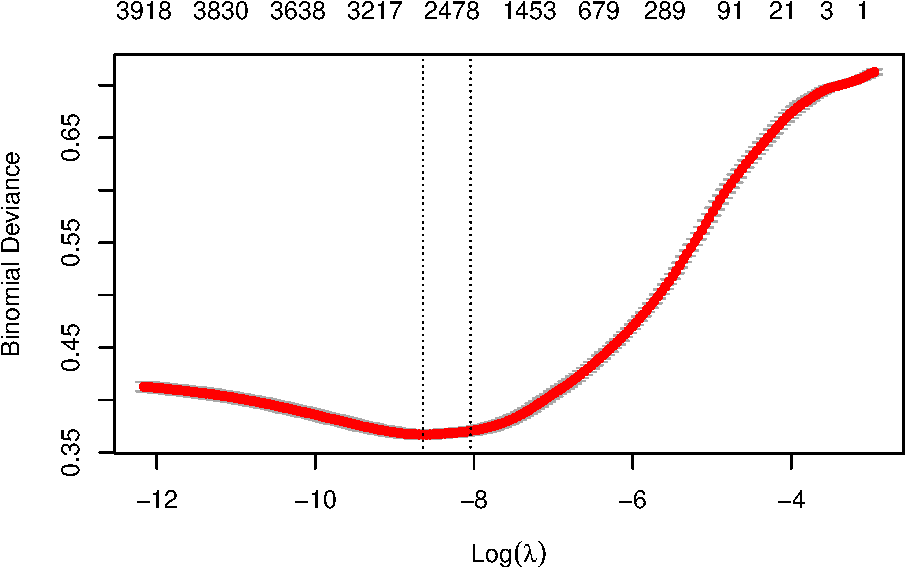
\includegraphics{classifier_files/figure-latex/lasso-1.pdf}

\begin{Shaded}
\begin{Highlighting}[]
\CommentTok{\# CV Error}
\CommentTok{\# Value of Lambda that minimises CV error  }
\FunctionTok{paste}\NormalTok{(}\StringTok{"The value of lambda that minimises CV error (MSE) is"}\NormalTok{, lasso\_cv}\SpecialCharTok{$}\NormalTok{lambda.min, }\StringTok{"at index"}\NormalTok{, }\FunctionTok{which.min}\NormalTok{(lasso\_cv}\SpecialCharTok{$}\NormalTok{cvm))}
\end{Highlighting}
\end{Shaded}

\begin{verbatim}
## [1] "The value of lambda that minimises CV error (MSE) is 0.000176004683934386 at index 124"
\end{verbatim}

\begin{Shaded}
\begin{Highlighting}[]
\FunctionTok{paste}\NormalTok{(}\StringTok{"The value of lambda that is 1 standard deviation away from the optimum lambda value is"}\NormalTok{, lasso\_cv}\SpecialCharTok{$}\NormalTok{lambda}\FloatTok{.1}\NormalTok{se)}
\end{Highlighting}
\end{Shaded}

\begin{verbatim}
## [1] "The value of lambda that is 1 standard deviation away from the optimum lambda value is 0.000321240844039881"
\end{verbatim}

\begin{Shaded}
\begin{Highlighting}[]
\FunctionTok{paste}\NormalTok{(}\StringTok{"The optimum CV error MSE is"}\NormalTok{, }\DecValTok{1} \SpecialCharTok{{-}}\NormalTok{ lasso\_cv}\SpecialCharTok{$}\NormalTok{cvm[}\FunctionTok{which}\NormalTok{(lasso\_cv}\SpecialCharTok{$}\NormalTok{lambda }\SpecialCharTok{==}\NormalTok{ lasso\_cv}\SpecialCharTok{$}\NormalTok{lambda.min)])}
\end{Highlighting}
\end{Shaded}

\begin{verbatim}
## [1] "The optimum CV error MSE is 0.632785288662436"
\end{verbatim}

\begin{Shaded}
\begin{Highlighting}[]
\CommentTok{\# Predicting in test set}
\NormalTok{lasso\_test\_preds }\OtherTok{\textless{}{-}} \FunctionTok{predict}\NormalTok{(lasso\_cv, test\_dfm, }\AttributeTok{type =} \StringTok{"class"}\NormalTok{)}

\NormalTok{lasso\_test\_preds }\SpecialCharTok{\%\textgreater{}\%}
  \FunctionTok{as.data.frame}\NormalTok{() }\SpecialCharTok{\%\textgreater{}\%}
  \FunctionTok{group\_by}\NormalTok{(lambda}\FloatTok{.1}\NormalTok{se) }\SpecialCharTok{\%\textgreater{}\%}
  \FunctionTok{summarise}\NormalTok{(}\AttributeTok{count =} \FunctionTok{n}\NormalTok{())}
\end{Highlighting}
\end{Shaded}

\begin{verbatim}
## # A tibble: 2 x 2
##   lambda.1se count
##   <chr>      <int>
## 1 0          29673
## 2 1           2265
\end{verbatim}

\begin{Shaded}
\begin{Highlighting}[]
\CommentTok{\# Writng File for Kaggle Submission}
\NormalTok{lasso\_answers }\OtherTok{\textless{}{-}} \FunctionTok{cbind}\NormalTok{(coms\_te}\SpecialCharTok{$}\NormalTok{rev\_id, lasso\_test\_preds)}
\FunctionTok{colnames}\NormalTok{(lasso\_answers) }\OtherTok{\textless{}{-}} \FunctionTok{c}\NormalTok{(}\StringTok{\textquotesingle{}rev\_id\textquotesingle{}}\NormalTok{, }\StringTok{\textquotesingle{}toxic\textquotesingle{}}\NormalTok{)}
\FunctionTok{write.csv}\NormalTok{(lasso\_answers, }\StringTok{\textquotesingle{}lasso\_answers.csv\textquotesingle{}}\NormalTok{, }\AttributeTok{row.names=}\ConstantTok{FALSE}\NormalTok{)}

\CommentTok{\# Creating CSV for feature selection}
\NormalTok{best.lambda }\OtherTok{\textless{}{-}} \FunctionTok{which}\NormalTok{(lasso\_cv}\SpecialCharTok{$}\NormalTok{lambda}\SpecialCharTok{==}\NormalTok{lasso\_cv}\SpecialCharTok{$}\NormalTok{lambda}\FloatTok{.1}\NormalTok{se)}

\NormalTok{beta }\OtherTok{\textless{}{-}}\NormalTok{ lasso\_cv}\SpecialCharTok{$}\NormalTok{glmnet.fit}\SpecialCharTok{$}\NormalTok{beta[,best.lambda]}

\DocumentationTok{\#\# identifying predictive features}
\NormalTok{lasso\_betas }\OtherTok{\textless{}{-}} \FunctionTok{data.frame}\NormalTok{(}\AttributeTok{coef =} \FunctionTok{as.numeric}\NormalTok{(beta),}
                \AttributeTok{word =} \FunctionTok{names}\NormalTok{(beta), }\AttributeTok{stringsAsFactors=}\NormalTok{F)}

\NormalTok{lasso\_betas }\OtherTok{\textless{}{-}}\NormalTok{ lasso\_betas[}\FunctionTok{order}\NormalTok{(lasso\_betas}\SpecialCharTok{$}\NormalTok{coef),]}

\FunctionTok{head}\NormalTok{(lasso\_betas[,}\FunctionTok{c}\NormalTok{(}\StringTok{"coef"}\NormalTok{, }\StringTok{"word"}\NormalTok{)], }\AttributeTok{n=}\DecValTok{10}\NormalTok{)}
\end{Highlighting}
\end{Shaded}

\begin{verbatim}
##           coef          word
## 2034 -6.187572        camera
## 515  -2.729750 continu_block
## 2284 -2.507863      want_add
## 3847 -2.424135 misunderstood
## 3093 -2.370612    messagebox
## 3589 -2.114716          dave
## 3492 -2.050632       default
## 861  -1.807590           cnn
## 1551 -1.784670  stop_continu
## 2025 -1.654772    pleas_help
\end{verbatim}

\begin{Shaded}
\begin{Highlighting}[]
\NormalTok{lasso\_betas }\OtherTok{\textless{}{-}}\NormalTok{ lasso\_betas[}\FunctionTok{order}\NormalTok{(lasso\_betas}\SpecialCharTok{$}\NormalTok{coef, }\AttributeTok{decreasing=}\ConstantTok{TRUE}\NormalTok{),]}

\FunctionTok{head}\NormalTok{(lasso\_betas[,}\FunctionTok{c}\NormalTok{(}\StringTok{"coef"}\NormalTok{, }\StringTok{"word"}\NormalTok{)], }\AttributeTok{n=}\DecValTok{10}\NormalTok{)}
\end{Highlighting}
\end{Shaded}

\begin{verbatim}
##          coef       word
## 2660 4.029593 motherfuck
## 384  3.657146       fuck
## 701  2.992526      idiot
## 692  2.974212     asshol
## 2407 2.965754     stupid
## 2890 2.791673    goddamn
## 1763 2.756463        wtf
## 3982 2.751383    dumbass
## 1704 2.581292       crap
## 1489 2.502146       suck
\end{verbatim}

\begin{Shaded}
\begin{Highlighting}[]
\FunctionTok{write.csv}\NormalTok{(lasso\_betas, }\StringTok{\textquotesingle{}lasso\_betas.csv\textquotesingle{}}\NormalTok{, }\AttributeTok{row.names=}\ConstantTok{FALSE}\NormalTok{)}

\NormalTok{lasso\_features\_to\_remove }\OtherTok{\textless{}{-}}\NormalTok{ lasso\_betas }\SpecialCharTok{\%\textgreater{}\%}
  \FunctionTok{filter}\NormalTok{(coef }\SpecialCharTok{==} \DecValTok{0}\NormalTok{) }\SpecialCharTok{\%\textgreater{}\%}
  \FunctionTok{select}\NormalTok{(word) }\SpecialCharTok{\%\textgreater{}\%}
  \FunctionTok{as.vector}\NormalTok{()}

\NormalTok{lasso\_features\_to\_remove }\OtherTok{\textless{}{-}}\NormalTok{ lasso\_features\_to\_remove[[}\DecValTok{1}\NormalTok{]]}

\CommentTok{\# LASSO Obsolete feature removal }
\CommentTok{\# Removing features where coefs went to 0. }

\NormalTok{dfm\_final }\OtherTok{\textless{}{-}}\NormalTok{ dfm\_final }\SpecialCharTok{\%\textgreater{}\%}
  \FunctionTok{dfm\_remove}\NormalTok{(}\AttributeTok{pattern =}\NormalTok{ lasso\_features\_to\_remove)}

\FunctionTok{paste}\NormalTok{(}\StringTok{"There are"}\NormalTok{, }\FunctionTok{ncol}\NormalTok{(dfm\_final), }\StringTok{"features after filtering via LASSO."}\NormalTok{)}
\end{Highlighting}
\end{Shaded}

\begin{verbatim}
## [1] "There are 2291 features after filtering via LASSO."
\end{verbatim}

\begin{Shaded}
\begin{Highlighting}[]
\DocumentationTok{\#\#\#\#\#\#\#\#\#\#\#\#\# Create test and train dfm sets.}
\NormalTok{train\_dfm }\OtherTok{\textless{}{-}}\NormalTok{ dfm\_final[dfm\_final}\SpecialCharTok{$}\NormalTok{sample }\SpecialCharTok{==} \StringTok{\textquotesingle{}train\textquotesingle{}}\NormalTok{,]}
\NormalTok{test\_dfm }\OtherTok{\textless{}{-}}\NormalTok{ dfm\_final[dfm\_final}\SpecialCharTok{$}\NormalTok{sample }\SpecialCharTok{==} \StringTok{\textquotesingle{}test\textquotesingle{}}\NormalTok{,]}

\CommentTok{\# Toxic vs. Non{-}toxic}
\NormalTok{toxic\_dfm }\OtherTok{\textless{}{-}}\NormalTok{ dfm\_final[train\_dfm}\SpecialCharTok{$}\NormalTok{toxic }\SpecialCharTok{==} \DecValTok{1}\NormalTok{, ]}
\end{Highlighting}
\end{Shaded}

\hypertarget{matrix-data-frame-manipulation}{%
\section{Matrix \& Data Frame
Manipulation}\label{matrix-data-frame-manipulation}}

\begin{Shaded}
\begin{Highlighting}[]
\FunctionTok{set.seed}\NormalTok{(}\DecValTok{1}\NormalTok{)}
\DocumentationTok{\#\#\#\#\#\#\#\#\#\#\#\#\#\#\#\#\#\#\# Train Data }

\CommentTok{\# Need to use \textquotesingle{}as\textquotesingle{} because data is so large that other functions dont work}
\NormalTok{train\_matrix }\OtherTok{\textless{}{-}} \FunctionTok{as}\NormalTok{(train\_dfm, }\StringTok{"Matrix"}\NormalTok{)}

\FunctionTok{colnames}\NormalTok{(train\_matrix) }\OtherTok{\textless{}{-}} \FunctionTok{colnames}\NormalTok{(train\_dfm)}

\NormalTok{cols\_train\_dfm }\OtherTok{\textless{}{-}} \FunctionTok{as.vector}\NormalTok{(}\FunctionTok{colnames}\NormalTok{(train\_dfm))}
\NormalTok{cols\_train\_matr }\OtherTok{\textless{}{-}} \FunctionTok{as.vector}\NormalTok{(}\FunctionTok{colnames}\NormalTok{(train\_matrix))}

\CommentTok{\#to clear physical memory}
\FunctionTok{rm}\NormalTok{(toks\_ngrams, dfm\_draft, dfm\_trimmed, cols\_train\_dfm, cols\_train\_matr)}

\CommentTok{\#Matrix to Data Frame manipulation}

\CommentTok{\# First convert to regular matrix }
\NormalTok{train\_matrix }\OtherTok{\textless{}{-}} \FunctionTok{as.matrix}\NormalTok{(train\_matrix)}

\CommentTok{\# doing this for computation reasons}

\CommentTok{\# convert to data frame}
\NormalTok{train\_df }\OtherTok{\textless{}{-}} \FunctionTok{as.data.frame}\NormalTok{(train\_matrix)}

\NormalTok{train\_x }\OtherTok{\textless{}{-}}\NormalTok{ train\_df}

\NormalTok{train\_y }\OtherTok{\textless{}{-}}\NormalTok{ coms\_tr}\SpecialCharTok{$}\NormalTok{toxic}

\CommentTok{\#add outcome variable to data frame}
\NormalTok{train\_df}\OtherTok{\textless{}{-}} \FunctionTok{cbind}\NormalTok{(train\_df, train\_y)}

\NormalTok{train\_df }\OtherTok{\textless{}{-}}\NormalTok{ train\_df }\SpecialCharTok{\%\textgreater{}\%}
  \FunctionTok{mutate}\NormalTok{(}\AttributeTok{train\_y =} \FunctionTok{as.factor}\NormalTok{(train\_y))}

\NormalTok{train\_df }\OtherTok{\textless{}{-}}\NormalTok{ train\_df }\SpecialCharTok{\%\textgreater{}\%}
  \FunctionTok{mutate}\NormalTok{(}\AttributeTok{train\_y =} \FunctionTok{factor}\NormalTok{(train\_y, }
                        \AttributeTok{labels =} \FunctionTok{make.names}\NormalTok{(}\FunctionTok{levels}\NormalTok{(train\_y))))}

\NormalTok{train\_df }\OtherTok{\textless{}{-}} \FunctionTok{clean\_names}\NormalTok{(train\_df)}

\CommentTok{\# Checking same length}
\FunctionTok{identical}\NormalTok{(}\FunctionTok{dim}\NormalTok{(train\_df)[}\DecValTok{1}\NormalTok{],}
\FunctionTok{length}\NormalTok{(train\_y))}
\end{Highlighting}
\end{Shaded}

\begin{verbatim}
## [1] TRUE
\end{verbatim}

\begin{Shaded}
\begin{Highlighting}[]
\NormalTok{train\_y }\OtherTok{\textless{}{-}} \FunctionTok{factor}\NormalTok{(train\_y)}

\NormalTok{train\_y }\OtherTok{\textless{}{-}} \FunctionTok{factor}\NormalTok{(train\_y, }\AttributeTok{labels =} \FunctionTok{make.names}\NormalTok{(}\FunctionTok{levels}\NormalTok{(train\_y)))}

\CommentTok{\# Matrix is too big}
\FunctionTok{rm}\NormalTok{(train\_matrix)}
\end{Highlighting}
\end{Shaded}

\hypertarget{toy-dataset}{%
\section{Toy Dataset}\label{toy-dataset}}

\begin{Shaded}
\begin{Highlighting}[]
\CommentTok{\# Create \textquotesingle{}sample\textquotesingle{} toy dataset }
\FunctionTok{set.seed}\NormalTok{(}\DecValTok{1}\NormalTok{)}

\NormalTok{sample\_index }\OtherTok{\textless{}{-}} \FunctionTok{sample}\NormalTok{(}\DecValTok{1}\SpecialCharTok{:}\FunctionTok{nrow}\NormalTok{(train\_df), }\FunctionTok{nrow}\NormalTok{(train\_df)}\SpecialCharTok{/}\DecValTok{10}\NormalTok{)}

\NormalTok{sample\_df }\OtherTok{\textless{}{-}}\NormalTok{ train\_df[sample\_index,]}

\NormalTok{sample\_x }\OtherTok{\textless{}{-}}\NormalTok{ train\_df[sample\_index,] }\SpecialCharTok{\%\textgreater{}\%}
  \FunctionTok{select}\NormalTok{(}\SpecialCharTok{{-}}\NormalTok{train\_y)}

\NormalTok{sample\_y }\OtherTok{\textless{}{-}}\NormalTok{ train\_df[sample\_index,] }\SpecialCharTok{\%\textgreater{}\%}
  \FunctionTok{select}\NormalTok{(train\_y) }

\CommentTok{\# create validation set within train for CV error}

\NormalTok{validation\_index }\OtherTok{\textless{}{-}} \FunctionTok{sample}\NormalTok{(}\DecValTok{1}\SpecialCharTok{:}\FunctionTok{nrow}\NormalTok{(train\_df), }\FunctionTok{nrow}\NormalTok{(train\_df)}\SpecialCharTok{/}\DecValTok{5}\NormalTok{)}

\NormalTok{validation\_x }\OtherTok{\textless{}{-}}\NormalTok{ train\_df[validation\_index,] }\SpecialCharTok{\%\textgreater{}\%}
  \FunctionTok{select}\NormalTok{(}\SpecialCharTok{{-}}\NormalTok{train\_y)}

\NormalTok{validation\_y }\OtherTok{\textless{}{-}}\NormalTok{ train\_df[validation\_index,] }\SpecialCharTok{\%\textgreater{}\%}
  \FunctionTok{select}\NormalTok{(train\_y) }

\CommentTok{\# create train without validation set.}

\NormalTok{train\_train\_x }\OtherTok{\textless{}{-}}\NormalTok{ train\_df[}\SpecialCharTok{{-}}\NormalTok{validation\_index,] }\SpecialCharTok{\%\textgreater{}\%}
  \FunctionTok{select}\NormalTok{(}\SpecialCharTok{{-}}\NormalTok{train\_y)}

\NormalTok{train\_train\_y }\OtherTok{\textless{}{-}}\NormalTok{ train\_df[}\SpecialCharTok{{-}}\NormalTok{validation\_index,] }\SpecialCharTok{\%\textgreater{}\%}
  \FunctionTok{select}\NormalTok{(train\_y) }
\end{Highlighting}
\end{Shaded}

\hypertarget{f1-function}{%
\section{F1 Function}\label{f1-function}}

\begin{Shaded}
\begin{Highlighting}[]
\NormalTok{calculate\_f1\_score }\OtherTok{\textless{}{-}} \ControlFlowTok{function}\NormalTok{(confusion\_matrix) \{}
  \CommentTok{\# Calculate the precision and recall}
\NormalTok{  true\_positives }\OtherTok{\textless{}{-}}\NormalTok{ confusion\_matrix[}\DecValTok{2}\NormalTok{,}\DecValTok{2}\NormalTok{]}
\NormalTok{  false\_positives }\OtherTok{\textless{}{-}}\NormalTok{ confusion\_matrix[}\DecValTok{1}\NormalTok{,}\DecValTok{2}\NormalTok{]}
\NormalTok{  false\_negatives }\OtherTok{\textless{}{-}}\NormalTok{ confusion\_matrix[}\DecValTok{2}\NormalTok{,}\DecValTok{1}\NormalTok{]}
  
\NormalTok{  precision }\OtherTok{\textless{}{-}}\NormalTok{ true\_positives }\SpecialCharTok{/}\NormalTok{ (true\_positives }\SpecialCharTok{+}\NormalTok{ false\_positives)}
\NormalTok{  recall }\OtherTok{\textless{}{-}}\NormalTok{ true\_positives }\SpecialCharTok{/}\NormalTok{ (true\_positives }\SpecialCharTok{+}\NormalTok{ false\_negatives)}
  
  \CommentTok{\# Calculate the F1 score}
\NormalTok{  f1\_score }\OtherTok{\textless{}{-}} \DecValTok{2} \SpecialCharTok{*}\NormalTok{ precision }\SpecialCharTok{*}\NormalTok{ recall }\SpecialCharTok{/}\NormalTok{ (precision }\SpecialCharTok{+}\NormalTok{ recall)}
  
  \FunctionTok{return}\NormalTok{(f1\_score)}
\NormalTok{\}}
\end{Highlighting}
\end{Shaded}

\hypertarget{exploratory-data-analysis}{%
\section{Exploratory Data Analysis}\label{exploratory-data-analysis}}

\begin{Shaded}
\begin{Highlighting}[]
\DocumentationTok{\#\#\#\#\#\#\#\#\#\#\#\#\#\# Feature Exploration }

\FunctionTok{textplot\_wordcloud}\NormalTok{(train\_dfm, }\AttributeTok{rotation=}\FloatTok{0.1}\NormalTok{, }\AttributeTok{random\_order =} \ConstantTok{FALSE}\NormalTok{, }\AttributeTok{min\_size=} \FloatTok{0.25}\NormalTok{, }\AttributeTok{max\_size=}\DecValTok{8}\NormalTok{, }\AttributeTok{min\_count =} \DecValTok{10}\NormalTok{, }\AttributeTok{max\_words=}\DecValTok{125}\NormalTok{, }\AttributeTok{color =} \StringTok{"red"}\NormalTok{)}
\end{Highlighting}
\end{Shaded}


\includegraphics{classifier_files/figure-latex/eda-1.pdf}

\begin{Shaded}
\begin{Highlighting}[]
\CommentTok{\# top features of train dfm}
\CommentTok{\# Using top features to remove words that are obsolete to prediction because they\textquotesingle{}re common across all comments. }
\FunctionTok{topfeatures}\NormalTok{(train\_dfm)}
\end{Highlighting}
\end{Shaded}

\begin{verbatim}
## pleas   one thank sourc   see think  also  know   get    go 
## 24363 24032 19456 19110 18287 17621 16613 16551 14472 14428
\end{verbatim}

\begin{Shaded}
\begin{Highlighting}[]
\NormalTok{top\_feats }\OtherTok{\textless{}{-}} \FunctionTok{names}\NormalTok{(}\FunctionTok{topfeatures}\NormalTok{(}\FunctionTok{fcm}\NormalTok{(train\_dfm), }\DecValTok{50}\NormalTok{))}

\FunctionTok{fcm}\NormalTok{(train\_dfm) }\SpecialCharTok{\%\textgreater{}\%}
  \FunctionTok{fcm\_select}\NormalTok{(}\AttributeTok{pattern =}\NormalTok{ top\_feats) }\SpecialCharTok{\%\textgreater{}\%}
  \FunctionTok{textplot\_network}\NormalTok{(}\AttributeTok{min\_freq =} \DecValTok{15}\NormalTok{, }\AttributeTok{edge\_color =} \StringTok{"orange"}\NormalTok{, }\AttributeTok{edge\_alpha =} \FloatTok{0.8}\NormalTok{, }\AttributeTok{edge\_size =} \DecValTok{1}\NormalTok{)}
\end{Highlighting}
\end{Shaded}

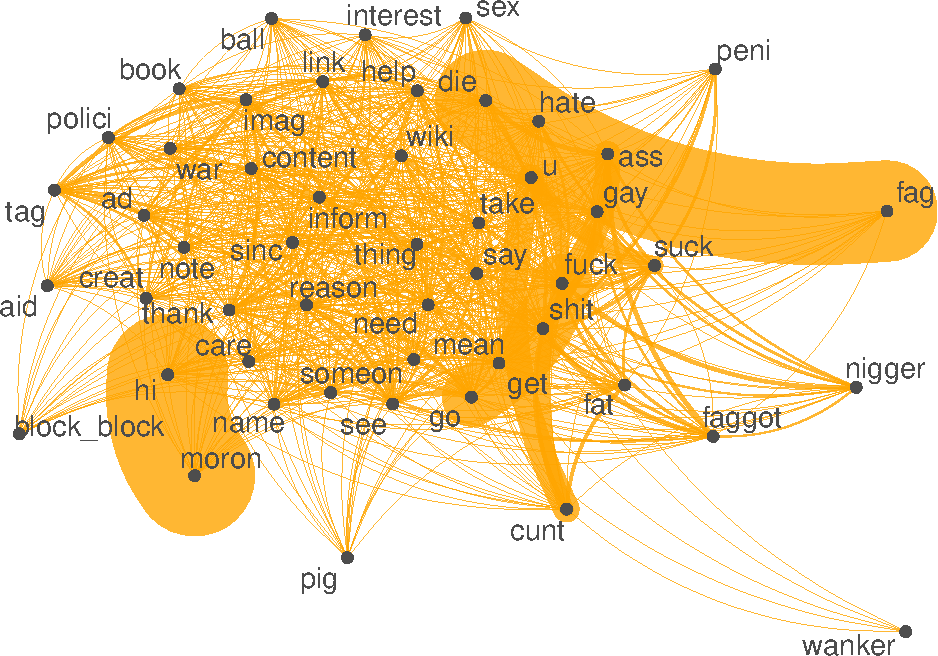
\includegraphics{classifier_files/figure-latex/eda-2.pdf}

\begin{Shaded}
\begin{Highlighting}[]
\DocumentationTok{\#\#\#\#\#\#\#\#\#\#\#\#\#\# Dispersion/Sparseness}
\FunctionTok{paste}\NormalTok{(}\StringTok{"Approximately"}\NormalTok{, }\DecValTok{1} \SpecialCharTok{{-}} \FunctionTok{sparsity}\NormalTok{(train\_dfm), }\StringTok{"of our train dfm contains non{-}zero frequency values, across"}\NormalTok{, }\FunctionTok{ncol}\NormalTok{(train\_dfm), }\StringTok{"features."}\NormalTok{)}
\end{Highlighting}
\end{Shaded}

\begin{verbatim}
## [1] "Approximately 0.00672792737808625 of our train dfm contains non-zero frequency values, across 2291 features."
\end{verbatim}

\begin{Shaded}
\begin{Highlighting}[]
\CommentTok{\# Even though its English Wiki {-} Are we sure that all the words are \textquotesingle{}English\textquotesingle{} or are there some slang words that aren\textquotesingle{}t recognised as English across texts?}
\NormalTok{TTR }\OtherTok{\textless{}{-}} \FunctionTok{textstat\_lexdiv}\NormalTok{(train\_dfm) }\SpecialCharTok{\%\textgreater{}\%}
  \FunctionTok{arrange}\NormalTok{(TTR) }

\FunctionTok{paste}\NormalTok{(}\StringTok{"The average lexical diversity across our training data is"}\NormalTok{, }\FunctionTok{mean}\NormalTok{(TTR}\SpecialCharTok{$}\NormalTok{TTR, }\AttributeTok{na.rm =} \ConstantTok{TRUE}\NormalTok{))}
\end{Highlighting}
\end{Shaded}

\begin{verbatim}
## [1] "The average lexical diversity across our training data is 0.901309234529594"
\end{verbatim}

\begin{Shaded}
\begin{Highlighting}[]
\DocumentationTok{\#\#\#\#\#\#\#\#\#\#\#\#\#\#\#\#\# Exploring Conditionals {-} Toxic vs. non{-}Toxic groups}

\DocumentationTok{\#\#\#\#\#\# Can we do a t.test for difference in means for length of toxic comments vs non{-}toxic comments?}

\NormalTok{coms\_tr}\SpecialCharTok{$}\NormalTok{length }\OtherTok{\textless{}{-}} \FunctionTok{nchar}\NormalTok{(coms\_tr}\SpecialCharTok{$}\NormalTok{comment)}

\NormalTok{(}\FunctionTok{mean}\NormalTok{(coms\_tr[coms\_tr}\SpecialCharTok{$}\NormalTok{toxic}\SpecialCharTok{==}\DecValTok{1}\NormalTok{,]}\SpecialCharTok{$}\NormalTok{length) }\SpecialCharTok{{-}} \FunctionTok{mean}\NormalTok{(coms\_tr[coms\_tr}\SpecialCharTok{$}\NormalTok{toxic}\SpecialCharTok{==}\DecValTok{0}\NormalTok{,]}\SpecialCharTok{$}\NormalTok{length))}
\end{Highlighting}
\end{Shaded}

\begin{verbatim}
## [1] -95.7614
\end{verbatim}

\begin{Shaded}
\begin{Highlighting}[]
\NormalTok{toxic\_len }\OtherTok{\textless{}{-}}\NormalTok{ coms\_tr}\SpecialCharTok{$}\NormalTok{length[coms\_tr}\SpecialCharTok{$}\NormalTok{toxic }\SpecialCharTok{==} \DecValTok{1}\NormalTok{]}

\NormalTok{non\_toxic\_len }\OtherTok{\textless{}{-}}\NormalTok{ coms\_tr}\SpecialCharTok{$}\NormalTok{length[coms\_tr}\SpecialCharTok{$}\NormalTok{toxic }\SpecialCharTok{==} \DecValTok{0}\NormalTok{]}

\NormalTok{t\_test\_result\_len }\OtherTok{\textless{}{-}} \FunctionTok{t.test}\NormalTok{(toxic\_len, non\_toxic\_len)}

\NormalTok{t\_test\_result\_len}
\end{Highlighting}
\end{Shaded}

\begin{verbatim}
## 
##  Welch Two Sample t-test
## 
## data:  toxic_len and non_toxic_len
## t = -18.166, df = 18549, p-value < 2.2e-16
## alternative hypothesis: true difference in means is not equal to 0
## 95 percent confidence interval:
##  -106.09410  -85.42871
## sample estimates:
## mean of x mean of y 
##  315.6897  411.4511
\end{verbatim}

\begin{Shaded}
\begin{Highlighting}[]
\CommentTok{\# print the p{-}value}
\FunctionTok{print}\NormalTok{(t\_test\_result\_len}\SpecialCharTok{$}\NormalTok{p.value)}
\end{Highlighting}
\end{Shaded}

\begin{verbatim}
## [1] 4.147762e-73
\end{verbatim}

\begin{Shaded}
\begin{Highlighting}[]
\DocumentationTok{\#\#\#\#\#\# Top Features for Toxic Data}
\FunctionTok{textplot\_wordcloud}\NormalTok{(toxic\_dfm, }\AttributeTok{rotation=}\DecValTok{0}\NormalTok{, }\AttributeTok{min\_size=}\NormalTok{.}\DecValTok{75}\NormalTok{, }\AttributeTok{max\_size=}\DecValTok{5}\NormalTok{, }\AttributeTok{max\_words=}\DecValTok{50}\NormalTok{)}
\end{Highlighting}
\end{Shaded}

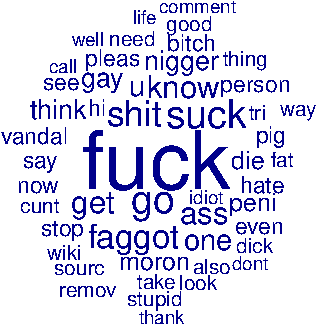
\includegraphics{classifier_files/figure-latex/eda-3.pdf}

\begin{Shaded}
\begin{Highlighting}[]
\CommentTok{\# Much different to top features for full dfm}
\FunctionTok{topfeatures}\NormalTok{(toxic\_dfm)}
\end{Highlighting}
\end{Shaded}

\begin{verbatim}
##   fuck     go   suck   shit faggot    get   know    ass      u    one 
##   9918   4097   3936   3419   3216   2920   2761   2752   2475   2398
\end{verbatim}

\begin{Shaded}
\begin{Highlighting}[]
\FunctionTok{rm}\NormalTok{(coms\_tr, zero\_tfidf, zero\_tfidf\_names)}
\end{Highlighting}
\end{Shaded}

\hypertarget{creating-validation-sets}{%
\section{Creating Validation Sets}\label{creating-validation-sets}}

\begin{Shaded}
\begin{Highlighting}[]
\FunctionTok{set.seed}\NormalTok{(}\DecValTok{1}\NormalTok{)}

\CommentTok{\# Creates tfidf scores on feature selected training set}
\NormalTok{tfidf\_data }\OtherTok{\textless{}{-}} \FunctionTok{dfm\_tfidf}\NormalTok{(train\_dfm, }\AttributeTok{scheme\_tf =} \StringTok{\textquotesingle{}prop\textquotesingle{}}\NormalTok{)}

\CommentTok{\# creating train index}
\NormalTok{N }\OtherTok{\textless{}{-}} \FunctionTok{floor}\NormalTok{(.}\DecValTok{8}\SpecialCharTok{*}\FunctionTok{nrow}\NormalTok{(tfidf\_data))}
\NormalTok{train\_idx }\OtherTok{\textless{}{-}} \FunctionTok{sample}\NormalTok{(}\DecValTok{1}\SpecialCharTok{:}\FunctionTok{nrow}\NormalTok{(tfidf\_data), N)}

\CommentTok{\# Creating train and test sets}
\NormalTok{train\_val }\OtherTok{\textless{}{-}}\NormalTok{ tfidf\_data[train\_idx,]}
\NormalTok{test\_val }\OtherTok{\textless{}{-}}\NormalTok{ tfidf\_data[}\SpecialCharTok{{-}}\NormalTok{train\_idx,]}

\NormalTok{toxic\_values\_train }\OtherTok{\textless{}{-}} \FunctionTok{docvars}\NormalTok{(train\_val)}\SpecialCharTok{$}\NormalTok{toxic}
\NormalTok{toxic\_values\_test }\OtherTok{\textless{}{-}} \FunctionTok{docvars}\NormalTok{(test\_val)}\SpecialCharTok{$}\NormalTok{toxic}
\end{Highlighting}
\end{Shaded}

\hypertarget{naive-bayes-classifier}{%
\section{Naive Bayes Classifier}\label{naive-bayes-classifier}}

\begin{Shaded}
\begin{Highlighting}[]
\DocumentationTok{\#\#\#\#\#\#\#\#\#\# Cross Validation of Naive Bayes Classifier for more accurate estimation of test error}

\CommentTok{\# Shuffle training data only}
\NormalTok{shuffle\_data\_indices }\OtherTok{\textless{}{-}} \FunctionTok{sample}\NormalTok{(}\DecValTok{1}\SpecialCharTok{:}\FunctionTok{nrow}\NormalTok{(train\_dfm))}

\CommentTok{\# Split training data into 10 folds}
\NormalTok{split\_data\_indices }\OtherTok{\textless{}{-}} \FunctionTok{split}\NormalTok{(shuffle\_data\_indices, }\FunctionTok{rep}\NormalTok{(}\DecValTok{1}\SpecialCharTok{:}\DecValTok{10}\NormalTok{, }\AttributeTok{length.out =} \FunctionTok{length}\NormalTok{(train\_val)))}

\CommentTok{\# Create empty vector for F1 score}
\NormalTok{nb\_f1\_score }\OtherTok{\textless{}{-}} \FunctionTok{c}\NormalTok{()}

\ControlFlowTok{for}\NormalTok{ (fold }\ControlFlowTok{in} \DecValTok{1}\SpecialCharTok{:}\DecValTok{10}\NormalTok{)\{}
    
  \CommentTok{\#split ONLY training data into respective training \& fold sets}
\NormalTok{  fold\_index }\OtherTok{\textless{}{-}}\NormalTok{ split\_data\_indices[[fold]]}
\NormalTok{  left\_out\_fold }\OtherTok{\textless{}{-}}\NormalTok{ train\_dfm[fold\_index,]}
\NormalTok{  train\_group }\OtherTok{\textless{}{-}}\NormalTok{ train\_dfm[}\SpecialCharTok{{-}}\NormalTok{fold\_index,]}
  
  \CommentTok{\# Train model}
\NormalTok{  nb\_mod }\OtherTok{\textless{}{-}} \FunctionTok{textmodel\_nb}\NormalTok{(}\AttributeTok{x =}\NormalTok{ train\_group, }\AttributeTok{y =} \FunctionTok{docvars}\NormalTok{(train\_group)}\SpecialCharTok{$}\NormalTok{toxic)}
  
  \CommentTok{\# predicting labels for validation fold }
\NormalTok{  nb\_preds }\OtherTok{\textless{}{-}} \FunctionTok{predict}\NormalTok{(nb\_mod, }\AttributeTok{newdata =}\NormalTok{ left\_out\_fold)}
  
  \CommentTok{\# computing the confusion matrix}
\NormalTok{  (nb\_cm }\OtherTok{\textless{}{-}} \FunctionTok{table}\NormalTok{(nb\_preds, }\FunctionTok{docvars}\NormalTok{(left\_out\_fold)}\SpecialCharTok{$}\NormalTok{toxic))}
  
  \CommentTok{\# Calculate F1 score}
\NormalTok{  fold\_f1 }\OtherTok{\textless{}{-}} \FunctionTok{calculate\_f1\_score}\NormalTok{(nb\_cm)}
  
\NormalTok{  nb\_f1\_score }\OtherTok{\textless{}{-}} \FunctionTok{c}\NormalTok{(nb\_f1\_score, fold\_f1)}
    
\NormalTok{\}}

\CommentTok{\# Vector of CV F1 scores}
\NormalTok{nb\_f1\_score}
\end{Highlighting}
\end{Shaded}

\begin{verbatim}
##  [1] 0.6482103 0.6673763 0.6491326 0.6467827 0.6459921 0.6530039 0.6687915
##  [8] 0.6264730 0.6619021 0.6523011
\end{verbatim}

\begin{Shaded}
\begin{Highlighting}[]
\CommentTok{\# Average CV F1 scores over 10 folds}
\FunctionTok{mean}\NormalTok{(nb\_f1\_score)}
\end{Highlighting}
\end{Shaded}

\begin{verbatim}
## [1] 0.6519966
\end{verbatim}

\begin{Shaded}
\begin{Highlighting}[]
\NormalTok{nb\_mod }\OtherTok{\textless{}{-}} \FunctionTok{textmodel\_nb}\NormalTok{(}\AttributeTok{x =}\NormalTok{ train\_dfm, }\AttributeTok{y =} \FunctionTok{docvars}\NormalTok{(train\_dfm)}\SpecialCharTok{$}\NormalTok{toxic)}

\NormalTok{nb\_y\_preds }\OtherTok{\textless{}{-}} \FunctionTok{predict}\NormalTok{(nb\_mod, test\_dfm, }\AttributeTok{type =} \StringTok{"class"}\NormalTok{)}

\CommentTok{\# Output answers for submission to Kaggle}
\NormalTok{nb\_answers }\OtherTok{\textless{}{-}} \FunctionTok{cbind}\NormalTok{(coms\_te}\SpecialCharTok{$}\NormalTok{rev\_id, nb\_y\_preds)}
\FunctionTok{colnames}\NormalTok{(nb\_answers) }\OtherTok{\textless{}{-}} \FunctionTok{c}\NormalTok{(}\StringTok{\textquotesingle{}rev\_id\textquotesingle{}}\NormalTok{, }\StringTok{\textquotesingle{}toxic\textquotesingle{}}\NormalTok{)}
\FunctionTok{write.csv}\NormalTok{(nb\_answers, }\StringTok{\textquotesingle{}nb\_answers.csv\textquotesingle{}}\NormalTok{, }\AttributeTok{row.names=}\ConstantTok{FALSE}\NormalTok{)}
\end{Highlighting}
\end{Shaded}

\hypertarget{support-vector-machine-svm}{%
\section{Support Vector Machine
(SVM)}\label{support-vector-machine-svm}}

\begin{Shaded}
\begin{Highlighting}[]
\DocumentationTok{\#\#\#\#\#\#\#\#\#\#\#\#\#\# SVM Cross Validation for Hyperparameter Tuning}

\CommentTok{\# Setting up parameter tuning process with grid search}
\NormalTok{evaluation }\OtherTok{\textless{}{-}} \FunctionTok{textmodel\_evaluate}\NormalTok{(}\AttributeTok{x =}\NormalTok{ train\_val, }\AttributeTok{y =}\NormalTok{ toxic\_values\_train,}
                                 \AttributeTok{k =} \DecValTok{3}\NormalTok{, }\AttributeTok{seed =} \DecValTok{1}\NormalTok{, }
                                 \AttributeTok{parameters =} \FunctionTok{list}\NormalTok{(}\AttributeTok{cost =} \FunctionTok{c}\NormalTok{(}\DecValTok{2}\NormalTok{, }\DecValTok{5}\NormalTok{, }\DecValTok{10}\NormalTok{), }\AttributeTok{epsilon =} \FunctionTok{c}\NormalTok{(}\FloatTok{0.01}\NormalTok{, }\FloatTok{0.05}\NormalTok{, }\FloatTok{0.1}\NormalTok{)),}
                                 \AttributeTok{model =} \StringTok{"textmodel\_svm"}\NormalTok{, }\AttributeTok{fun =} \StringTok{"f1\_score"}\NormalTok{)}

\CommentTok{\# Assessing Hyperparameter Optimisation Grid Search }
\FunctionTok{head}\NormalTok{(evaluation)}
\end{Highlighting}
\end{Shaded}

\begin{verbatim}
##   k  f1_score cost epsilon  time seed
## 1 1 0.8440932    2    0.01 15.94    1
## 2 2 0.8427954    2    0.01 17.62    1
## 3 3 0.8470240    2    0.01 14.05    1
## 4 1 0.8449624    5    0.01 29.35    1
## 5 2 0.8450412    5    0.01 27.15    1
\end{verbatim}

\begin{Shaded}
\begin{Highlighting}[]
\CommentTok{\# Finding the best HP value for cost}
\NormalTok{cost\_hp }\OtherTok{\textless{}{-}} \FunctionTok{aggregate}\NormalTok{(evaluation, }\AttributeTok{by =} \FunctionTok{list}\NormalTok{(evaluation}\SpecialCharTok{$}\NormalTok{cost), }\AttributeTok{FUN =} \StringTok{"mean"}\NormalTok{)}
\NormalTok{cost\_hp}
\end{Highlighting}
\end{Shaded}

\begin{verbatim}
##   Group.1 k  f1_score cost    epsilon     time seed
## 1       2 2 0.8446375    2 0.05333333 11.50111    1
## 2       5 2 0.8457353    5 0.05333333 20.15222    1
## 3      10 2 0.8466549   10 0.05333333 32.88111    1
\end{verbatim}

\begin{Shaded}
\begin{Highlighting}[]
\NormalTok{cost\_best\_idx }\OtherTok{\textless{}{-}} \FunctionTok{which.max}\NormalTok{(cost\_hp[,}\StringTok{\textquotesingle{}f1\_score\textquotesingle{}}\NormalTok{])}

\NormalTok{cost\_best }\OtherTok{\textless{}{-}}\NormalTok{ cost\_hp[cost\_best\_idx,}\StringTok{\textquotesingle{}Group.1\textquotesingle{}}\NormalTok{]}
\NormalTok{cost\_best}
\end{Highlighting}
\end{Shaded}

\begin{verbatim}
## [1] 10
\end{verbatim}

\begin{Shaded}
\begin{Highlighting}[]
\CommentTok{\# Finding the best HP value for epsilon}
\NormalTok{eps\_hp }\OtherTok{\textless{}{-}} \FunctionTok{aggregate}\NormalTok{(evaluation, }\AttributeTok{by =} \FunctionTok{list}\NormalTok{(evaluation}\SpecialCharTok{$}\NormalTok{epsilon), }\AttributeTok{FUN =} \StringTok{"mean"}\NormalTok{)}
\NormalTok{eps\_hp}
\end{Highlighting}
\end{Shaded}

\begin{verbatim}
##   Group.1 k  f1_score     cost epsilon     time seed
## 1    0.01 2 0.8456394 5.666667    0.01 26.18000    1
## 2    0.05 2 0.8456920 5.666667    0.05 20.71667    1
## 3    0.10 2 0.8456963 5.666667    0.10 17.63778    1
\end{verbatim}

\begin{Shaded}
\begin{Highlighting}[]
\NormalTok{eps\_best\_idx }\OtherTok{\textless{}{-}} \FunctionTok{which.max}\NormalTok{(eps\_hp[,}\StringTok{\textquotesingle{}f1\_score\textquotesingle{}}\NormalTok{])}
\NormalTok{eps\_best\_idx}
\end{Highlighting}
\end{Shaded}

\begin{verbatim}
## [1] 3
\end{verbatim}

\begin{Shaded}
\begin{Highlighting}[]
\NormalTok{eps\_best }\OtherTok{\textless{}{-}}\NormalTok{ eps\_hp[eps\_best\_idx,}\StringTok{\textquotesingle{}Group.1\textquotesingle{}}\NormalTok{]}
\NormalTok{eps\_best}
\end{Highlighting}
\end{Shaded}

\begin{verbatim}
## [1] 0.1
\end{verbatim}

\begin{Shaded}
\begin{Highlighting}[]
\DocumentationTok{\#\#\#\#\#\#\#\#\#\#\# SVM Cross Validation for Estimation of Test Error}

\NormalTok{svm\_f1\_scores }\OtherTok{\textless{}{-}} \FunctionTok{c}\NormalTok{()}

\ControlFlowTok{for}\NormalTok{ (fold }\ControlFlowTok{in} \DecValTok{1}\SpecialCharTok{:}\DecValTok{4}\NormalTok{)\{}
    
  \CommentTok{\#split ONLY training data into respective training \& fold sets}
\NormalTok{  fold\_index }\OtherTok{\textless{}{-}}\NormalTok{ split\_data\_indices[[fold]]}
\NormalTok{  left\_out\_fold }\OtherTok{\textless{}{-}}\NormalTok{ train\_dfm[fold\_index,]}
\NormalTok{  train\_group }\OtherTok{\textless{}{-}}\NormalTok{ train\_dfm[}\SpecialCharTok{{-}}\NormalTok{fold\_index,]}
  
  \CommentTok{\# Train model}
\NormalTok{  svm\_best\_mod\_cv }\OtherTok{\textless{}{-}} \FunctionTok{textmodel\_svm}\NormalTok{(}\AttributeTok{x =}\NormalTok{ train\_group, }\AttributeTok{y =} \FunctionTok{docvars}\NormalTok{(train\_group)}\SpecialCharTok{$}\NormalTok{toxic, }
                        \AttributeTok{cost =}\NormalTok{ cost\_best, }\AttributeTok{epsilon =}\NormalTok{ eps\_best)  }
  
  \CommentTok{\# predicting labels for validation fold }
\NormalTok{  svm\_y\_pred\_cv }\OtherTok{\textless{}{-}} \FunctionTok{predict}\NormalTok{(svm\_best\_mod\_cv, }\AttributeTok{newdata =}\NormalTok{ left\_out\_fold, }\AttributeTok{type =} \StringTok{"class"}\NormalTok{)}
  
  \CommentTok{\# computing the confusion matrix}
\NormalTok{  (svm\_cm }\OtherTok{\textless{}{-}} \FunctionTok{table}\NormalTok{(svm\_y\_pred\_cv, }\FunctionTok{docvars}\NormalTok{(left\_out\_fold)}\SpecialCharTok{$}\NormalTok{toxic))}
  
  \CommentTok{\# Calculate F1 score}
\NormalTok{  fold\_f1 }\OtherTok{\textless{}{-}} \FunctionTok{calculate\_f1\_score}\NormalTok{(svm\_cm)}
  
\NormalTok{  svm\_f1\_scores }\OtherTok{\textless{}{-}} \FunctionTok{c}\NormalTok{(svm\_f1\_scores, fold\_f1)}
    
\NormalTok{\}}

\NormalTok{svm\_f1\_scores}
\end{Highlighting}
\end{Shaded}

\begin{verbatim}
## [1] 0.7441673 0.7416144 0.7293263 0.7459334
\end{verbatim}

\begin{Shaded}
\begin{Highlighting}[]
\FunctionTok{mean}\NormalTok{(svm\_f1\_scores)}
\end{Highlighting}
\end{Shaded}

\begin{verbatim}
## [1] 0.7402604
\end{verbatim}

\begin{Shaded}
\begin{Highlighting}[]
\FunctionTok{paste}\NormalTok{(}\StringTok{"The CV Error for our Optimised SVM model is"}\NormalTok{, }\FunctionTok{mean}\NormalTok{(svm\_f1\_scores))}
\end{Highlighting}
\end{Shaded}

\begin{verbatim}
## [1] "The CV Error for our Optimised SVM model is 0.74026037806918"
\end{verbatim}

\begin{Shaded}
\begin{Highlighting}[]
\FunctionTok{paste}\NormalTok{(}\StringTok{"Our Optimised SVM model has a cost hyperparameter value of"}\NormalTok{, cost\_best)}
\end{Highlighting}
\end{Shaded}

\begin{verbatim}
## [1] "Our Optimised SVM model has a cost hyperparameter value of 10"
\end{verbatim}

\begin{Shaded}
\begin{Highlighting}[]
\FunctionTok{paste}\NormalTok{(}\StringTok{"Our Optimised SVM model has a epsilon hyperparameter value of"}\NormalTok{, eps\_best)}
\end{Highlighting}
\end{Shaded}

\begin{verbatim}
## [1] "Our Optimised SVM model has a epsilon hyperparameter value of 0.1"
\end{verbatim}

\begin{Shaded}
\begin{Highlighting}[]
\DocumentationTok{\#\#\#\#\#\#\#\#\#\#\# New model with Optimised HPs}
\NormalTok{svm\_best\_mod }\OtherTok{\textless{}{-}} \FunctionTok{textmodel\_svm}\NormalTok{(}\AttributeTok{x =}\NormalTok{ train\_val, }\AttributeTok{y =}\NormalTok{ toxic\_values\_train, }
                        \AttributeTok{cost =}\NormalTok{ cost\_best, }\AttributeTok{epsilon =}\NormalTok{ eps\_best)}

\NormalTok{svm\_y\_preds }\OtherTok{\textless{}{-}} \FunctionTok{predict}\NormalTok{(svm\_best\_mod, test\_dfm, }\AttributeTok{type =} \StringTok{"class"}\NormalTok{)}

\FunctionTok{paste}\NormalTok{(}\StringTok{"Our optimised SVM model predicts that"}\NormalTok{, }\FunctionTok{sum}\NormalTok{(svm\_y\_preds)}\SpecialCharTok{/}\FunctionTok{length}\NormalTok{(svm\_y\_preds), }\StringTok{"\% of the test set is toxic"}\NormalTok{)}
\end{Highlighting}
\end{Shaded}

\begin{verbatim}
## [1] "Our optimised SVM model predicts that 0.146346045463085 % of the test set is toxic"
\end{verbatim}

\begin{Shaded}
\begin{Highlighting}[]
\CommentTok{\# Output answers for submission to Kaggle}
\NormalTok{svm\_answers }\OtherTok{\textless{}{-}} \FunctionTok{cbind}\NormalTok{(coms\_te}\SpecialCharTok{$}\NormalTok{rev\_id, svm\_y\_preds)}
\FunctionTok{colnames}\NormalTok{(svm\_answers) }\OtherTok{\textless{}{-}} \FunctionTok{c}\NormalTok{(}\StringTok{\textquotesingle{}rev\_id\textquotesingle{}}\NormalTok{, }\StringTok{\textquotesingle{}toxic\textquotesingle{}}\NormalTok{)}
\FunctionTok{write.csv}\NormalTok{(svm\_answers, }\StringTok{\textquotesingle{}svm\_answers.csv\textquotesingle{}}\NormalTok{, }\AttributeTok{row.names=}\ConstantTok{FALSE}\NormalTok{)}
\end{Highlighting}
\end{Shaded}

\hypertarget{random-forest-rf}{%
\section{Random Forest (RF)}\label{random-forest-rf}}

\begin{Shaded}
\begin{Highlighting}[]
\CommentTok{\# Training on Sample for Variable Importance}

\CommentTok{\# rf\_gridsearch\_samp \textless{}{-} randomForest(x = sample\_x,  }
\CommentTok{\#                                   y = sample\_y$train\_y,}
\CommentTok{\#                                   ntree = 50,}
\CommentTok{\#                                   mtry = floor(sqrt(ncol(sample\_x))))}

\CommentTok{\# varImpPlot(rf\_gridsearch\_samp)}

\CommentTok{\# rf\_samp\_preds \textless{}{-} predict(rf\_gridsearch\_samp, validation\_x)}

\CommentTok{\# confusionMatrix(rf\_samp\_preds, factor(validation\_y$train\_y))}

\CommentTok{\# Training on Training data for final Random Forest Model}
\CommentTok{\# UNABLE TO DO SO DUE TO COMPUTING RESOURCES.}

\CommentTok{\# rf\_gridsearch \textless{}{-} randomForest(x = train\_train\_x, }
\CommentTok{\#                              y = train\_train\_y$train\_y, }
\CommentTok{\#                              ntree = 50, }
\CommentTok{\#                              mtry = floor(sqrt(ncol(train\_train\_x))))}

\CommentTok{\# varImpPlot(rf\_gridsearch)}

\CommentTok{\# Use model to predict in validation set}
\CommentTok{\# rf\_val\_preds \textless{}{-} predict(rf\_gridsearch, validation\_x)}
\end{Highlighting}
\end{Shaded}


\end{document}
